\documentclass{article}

\usepackage{graphicx}
\usepackage{tikz}
\usepackage{tikzsymbols}
\usetikzlibrary{calc,patterns,shapes.geometric}
\pagestyle{empty}
\usepackage[margin=0pt]{geometry}
\geometry{papersize={14in,12in}}

\def\centerarc[#1](#2)(#3:#4:#5){\draw[#1] ($(#2)+({#5*cos(#3)},{#5*sin(#3)})$) arc (#3:#4:#5);}

\begin{document}
	\begin{figure}
		\centering
		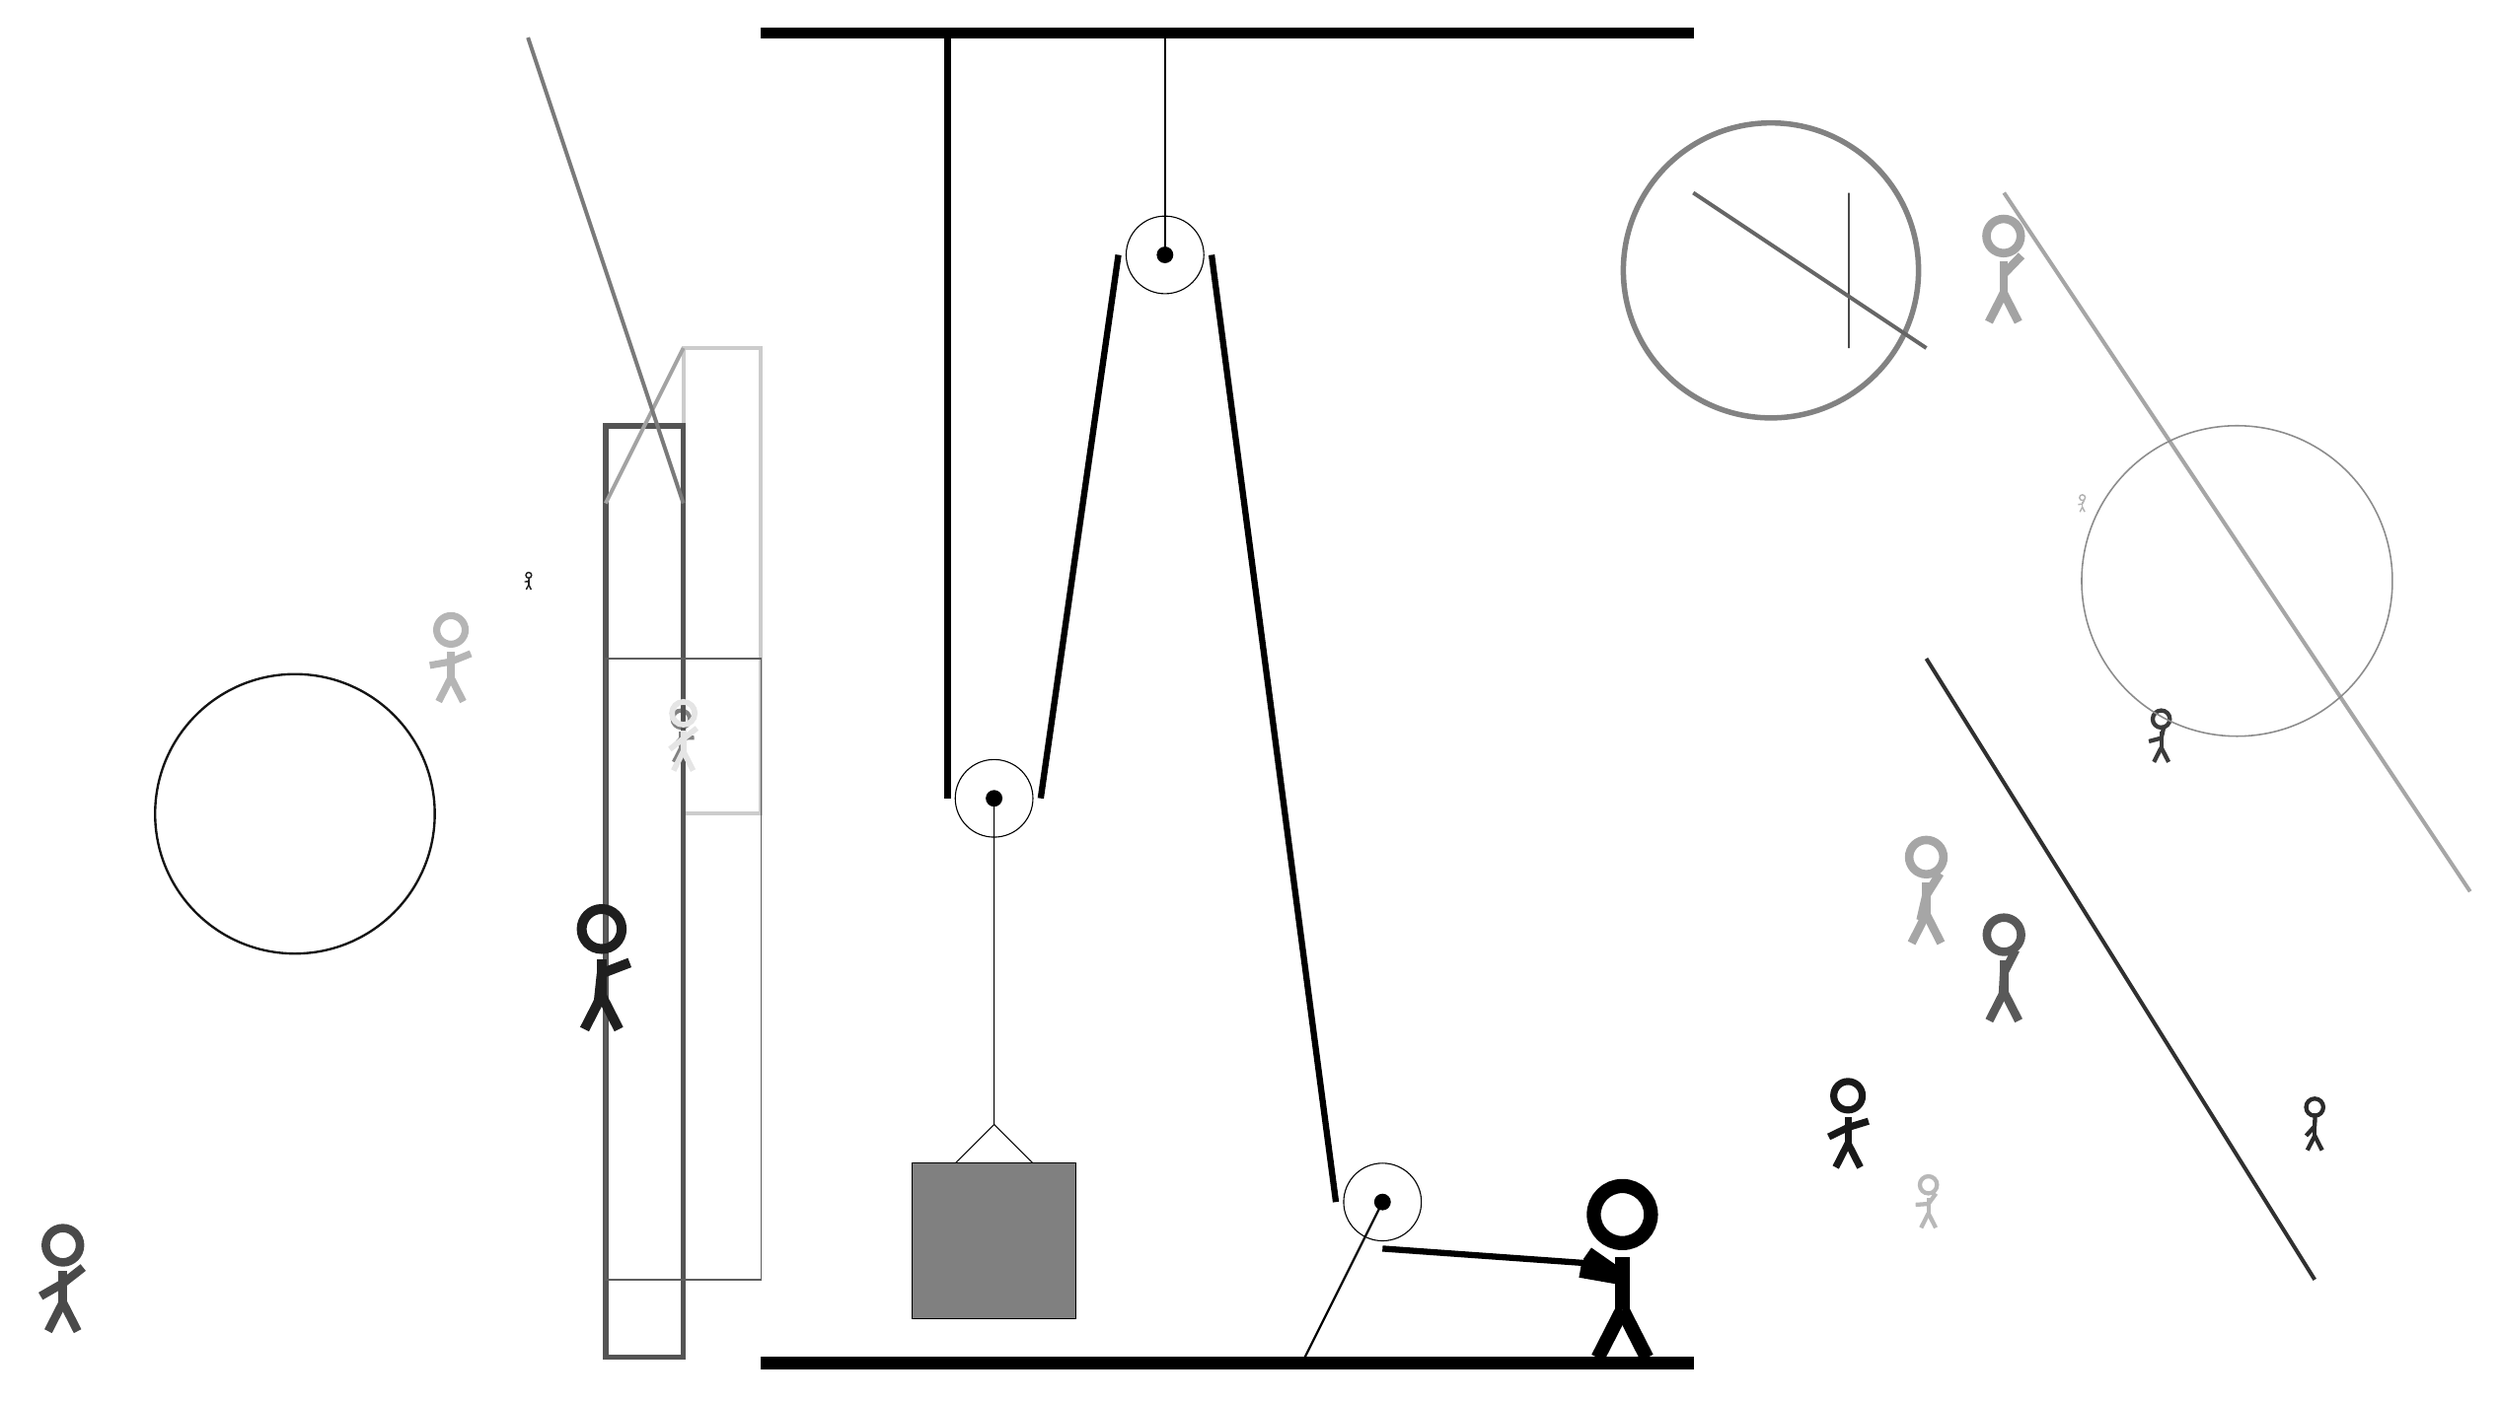
\begin{tikzpicture}
			%%%%% START %%%%%
			
			\draw[fill=black] (-2, 14) rectangle (10, 14.125);
			
			\draw (3.2, 11.2) circle (0.5);
			\draw[fill=black] (3.2, 11.2) circle (0.1);
			\draw[thick] (3.2, 11.2) -- (3.2, 14);
			
			\draw (6, -1) circle (0.5);
			\draw[fill=black] (6, -1) circle (0.1);
			\draw[thick] (6, -1) -- (5, -3);
			
			\draw (1, 4.2) circle (0.5);
			\draw[fill=black] (1, 4.2) circle (0.1);
			
			\draw (1, 4.2) -- (1, 0) -- (0.5, -0.5);
			\draw (1, 0) -- (1.5, -0.5);
			\draw[fill=black!50] (-0.05, -0.5) rectangle (2.05, -2.5);
			
			\draw[line width=0.8mm] (0.4, 14) -- (0.4, 4.2);
			\centerarc[line width=0.8mm](1, 4.2)(180:360:0.6);
			\draw[line width=0.8mm](1.6, 4.2) -- (2.6, 11.2);
			\centerarc[line width=0.8mm](3.2, 11.2)(0:180:0.6);
			\draw[line width=0.8mm](3.8, 11.2) -- (5.4, -1);
			\centerarc[line width=0.8mm](6, -1)(180:270:0.6);
			\draw[line width=0.8mm](6, -1.6) -- (8.8, -1.8);
			
			\node at (9, -1.9) {\Strichmaxerl[10][-35][170]};
			
			\draw[line width=0.5mm, color=black!35](14, 12) -- (20, 3);
			
			\draw[line width=0.5mm, color=black!20] (-2, 10) rectangle (-3, 4);
			\node[line width=0.5mm, color=black!49] at (-3, 5) {\Strichmaxerl[3][48][2]};
			\node[line width=0.6mm, color=black!83] at (18, 0) {\Strichmaxerl[3][48][88]};
			
			\node[line width=0.6mm, color=black!87] at (-5, 7) {\Strichmaxerl[1][2][85]};
			\node[line width=0.3mm, color=black!28] at (13, -1) {\Strichmaxerl[3][4][54]};
			\node[line width=0.6mm, color=black!77] at (16, 5) {\Strichmaxerl[3][15][77]};
			\draw[line width=0.7mm, color=black!67] (-3, -3) rectangle (-4, 9);
			\node[line width=0.3mm, color=black!90] at (12, 0) {\Strichmaxerl[5][26][17]};
			
			\draw[line width=0.2mm, color=black!63] (-4, 6) rectangle (-2, -2);
			
			\node[line width=0.6mm, color=black!71] at (-11, -2) {\Strichmaxerl[6][30][38]};
			
			\draw [line width=0.2mm, color=black!45](17, 7) circle (2.0);
			\node[line width=0.2mm, color=black!65] at (14, 2) {\Strichmaxerl[6][87][63]};
			
			\node[line width=0.5mm, color=black!30] at (15, 8) {\Strichmaxerl[1][8][63]};
			\draw[line width=0.5mm, color=black!36](-3, 10) -- (-4, 8);
			\node[line width=0.6mm, color=black!88] at (-4, 2) {\Strichmaxerl[7][84][21]};
			
			\draw [line width=0.6mm, color=black!33](-5, 12) circle (0.0);
			\draw [line width=0.7mm, color=black!49](11, 11) circle (1.9);
			\node[line width=0.4mm, color=black!35] at (13, 3) {\Strichmaxerl[6][77][58]};
			\node[line width=0.6mm, color=black!10] at (-3, 5) {\Strichmaxerl[4][38][38]};
			\draw[line width=0.3mm, color=black!71] (12, 12) rectangle (12, 10);
			
			\draw[line width=0.5mm, color=black!60](10, 12) -- (13, 10);
			\draw[line width=0.5mm, color=black!81](13, 6) -- (18, -2);
			\draw[line width=0.5mm, color=black!52](-5, 14) -- (-3, 8);
			\node[line width=0.4mm, color=black!29] at (-6, 6) {\Strichmaxerl[5][10][22]};
			\node[line width=0.3mm, color=black!36] at (14, 11) {\Strichmaxerl[6][90][46]};
			\draw [line width=0.3mm, color=black!92](-8, 4) circle (1.8);
			
			\draw[fill=black] (-2, -3) rectangle (10, -3.15);
			
			%%%%% END %%%%%
		\end{tikzpicture}
	\end{figure}	
\end{document}